% Created 2020-12-05 Sat 20:57
% Intended LaTeX compiler: pdflatex
\documentclass{article}
\usepackage[utf8]{inputenc}
\usepackage[T1]{fontenc}
\usepackage{graphicx}
\usepackage{grffile}
\usepackage{longtable}
\usepackage{wrapfig}
\usepackage{rotating}
\usepackage[normalem]{ulem}
\usepackage{amsmath}
\usepackage{textcomp}
\usepackage{amssymb}
\usepackage{capt-of}
\usepackage{hyperref}
\bibliographystyle{plain}
\author{Keagan McMahon, Brigitta Munds, \\ Benjamin Brown, \& Christina Rachmadita}
\date{\textit{<2020-12-14 Mon>} December 14th, 2020}
\title{PSYCH 363 - Stroop Effect: Congruency and Response Time}
\hypersetup{
 pdfauthor={Keagan McMahon, Brigitta Munds, \\ Benjamin Brown, \& Christina Rachmadita},
 pdftitle={PSYCH 363 - Stroop Effect: Congruency and Response Time},
 pdfkeywords={},
 pdfsubject={},
 pdfcreator={Emacs 26.3 (Org mode 9.1.9)}, 
 pdflang={English}}
\begin{document}

\maketitle
\tableofcontents

This is to test your installation of the files and programs needed to make a simple report. To compile to pdf use \texttt{C-c C-e l p}.

\section{Introduction}
\label{sec:org204155e}

Insert introduction text here\ldots{}


\section{Methods}
\label{sec:org10a27a8}

Insert some method text here

This loads an R library
\begin{verbatim}
library(random)
\end{verbatim}


\section{Results}
\label{sec:org17b9d7d}

Insert some results text here and other content (i.e. code, etc)

Now we will see if we can some source code and a simple plot for our export.

\begin{verbatim}
x = 1:10
y = rnorm(10)
print(mean(y))
\end{verbatim}

\begin{verbatim}
0.0938086862415748
\end{verbatim}

Here is some more R source code!
\begin{verbatim}
{ a=2
  b=6
  multiply <- function(a,b)
  return(a * b)
  print(paste(a, "multiplied by", b, "is", (print(multiply(a,b)))))
}

{ for(i in seq(1,10))
if(i%%2==0){ 
print(i) }
}
\end{verbatim}

Now lets try some Python source code from my loop assignment\ldots{}

\begin{verbatim}
letters = ['t', 'r', 'i', 'b', 'q', 'v', 'h', 'p']
position = ['1st', '2nd', '3rd', '4th', '5th', '6th', '7th', '8th']

for x in letters:
  print(x)

for i in sorted(letters):
  print(i)

for x in enumerate(zip(letters, position)):
  print("The {0} letter in list 1 is {0}".format(x))

\end{verbatim}


Here is a graph of our results for you to see: 

\begin{verbatim}
plot(x,y,type = 'b')
\end{verbatim}

\begin{center}
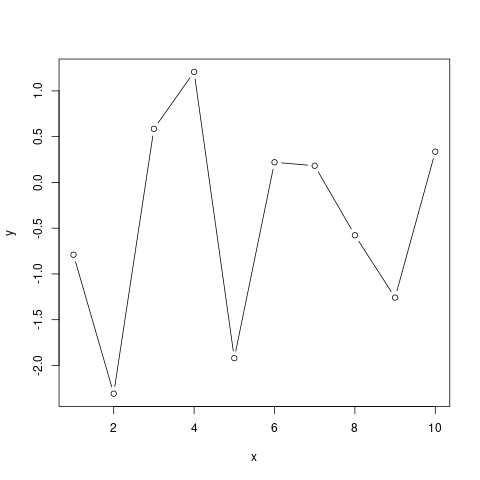
\includegraphics[width=.9\linewidth]{simplePlot.png}
\end{center}


Here is some code that produces a table of data for us:
\begin{verbatim}
d <- data.frame(foo=c('a','b','n'), bar=c(1.0/3.0,22,32))

d

\end{verbatim}

\begin{center}
\begin{tabular}{lr}
foo & bar\\
\hline
a & 0.333333333333333\\
b & 22\\
n & 32\\
\end{tabular}
\end{center}



Here is an example of an inline piece of code, it will generate 20 random numbers:
\begin{verbatim}

xinline = rnorm(20)

\end{verbatim}

We can use that code in this way:

The mean of 20 mean 0 normally distributed numbers is -0.3251309856653.


\section{Conclusions}
\label{sec:orgebe2160}

Put some type of conlusion content here\ldots{}.



\section{References}
\label{sec:org8633c68}

Insert some references here, such as\ldots{}

This article \cite{britt}

\bibliography{stroopBib.bib}


\section{Testing Plots here\ldots{}..}
\label{sec:orgdd5fd9f}
\begin{verbatim}
library(ggplot2)

data <- read.csv("/home/keagan/GitRepos/363Stroop/363Stroop_Data_Dec_4.csv")

incongruent <- data[which(data$Congruent == 0),]$Time
congruent <- data[which(data$Congruent == 1),]$Time
df <- data.frame(cond = c("Incongruent", "Congruent"), rt = c(mean(incongruent), mean(congruent)))

p <- ggplot(df, aes(x = cond, y = rt, fill = cond)) + geom_bar(stat = "identity", width = 0.5) + labs(title = "Condition on Reaction Time", x = "Condition", y = "Reaction Time (s)") + theme(legend.position = "right") + theme_minimal()
p
\end{verbatim}

\begin{center}
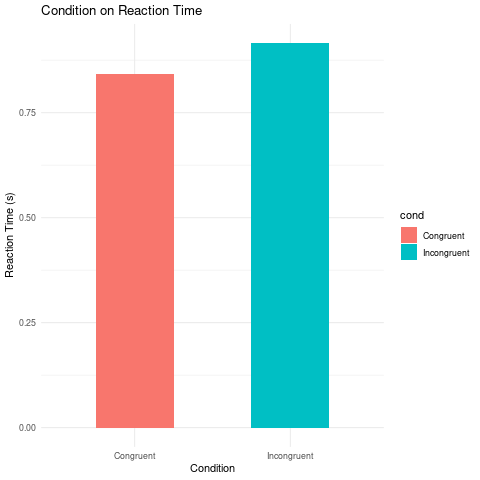
\includegraphics[width=.9\linewidth]{barplot_stroop.png}
\end{center}
\end{document}
